\section{Introduction}

% Bring in the issues that our approach can address
% Describe them as problems in current simulation/emulation systems
Software defined networking (SDN) explicitly separate the logic of the network
from the distributed hardware that implementing the forwarding behaviors.
This centralized scheme have been widely adopted in datacenters networks
and internet exchange points\cite{B4, Meridian, SDX}.
However, similar to traditional computer network systems, it is still crucial to do testing
and evaluating before deployment.
Consequently researchers in the simulation community have extend various
traditional network simulators to provide SDN support\cite{S3F, NS3, OPNET}.
Though network simulation is both reproducible and scalable,
people are not always confident with its fidelity due to its idealized modelling process.
In contrast, researcher in SDN community propose container-based emulation that utilize
shared hardware resources and real network stack to run high-fidelity SDN experiments\cite{Mininet}.
However, the experiment scale is limited to the resources available on the running machine.
For example in a traditional tree-topology network with depth 4 and fanout 10,
we need to start up 1111 switches and 10000 hosts.
If we want to achieve full connectivity, we need to install at least 399,960,000($\approx$ 4 * 10000 * 9999)
OpenFlow rules in total.
Assuming rules only have source IP address, destination IP address, inport number and outport number,
each rule will consume at least 10 Bytes memory, meaning around 3.72 GB of memory are required to
emulate this network.
Such intensive resource requirement are not commonly satisfied by commodity low-end machines.

% State our idea
In this work we propose to address the scalability issue by simplifying the emulated
SDN network both logically and physically.
Inspired by works of~\cite{OneBigSwitchAbstraction},
we abstract a subset of the networked SDN switches as \textbf{one} big switch.
The one big switch idea in~\cite{OneBigSwitchAbstraction} abstracts the entire SDN network as
a big switch so that the network applications just need to programme the network with simple
endpoint policy, while the controller platform is helping in the background to handle
the low-level problems such as routing policy, switch memory limits and forwarding rules.
Our idea is to apply the big switch abstraction reversely:
if the user of network emulation are just interested in the behavior of the packets in
a snapshot of the network, but not interested in what happened in the bottom of the network,
for example, hop-by-hop routing rule, memory consumption on the switch, then why don't we
just create a network with only endpoint policy and emulate it such that packet-level
fidelity is preserved.
In this case, we can compress the entire set of the SDN switches to single OpenFlow switch.

The obvious benefit is the much less number of switches and/or number of rules existing in the network.
For the example mention above, we only need to start up one switch and 10000 hosts.
On the single switch, we just need to install about 99,990,000 rules, only requiring less than 0.94 GB memory.
Besides, the abstracted big switch can be used in multiple plug-in-play scenarios.
For example, researchers can reproduce the simulation result with very
simple configurations (link connectivity setup, flow table configuration etc.)
after one complex run on the original network.
In the case of a too-large-to-simulate network, we can divide it into subsets of switches,
abstract each subset separately.
Then we are able to combine multiple ``big switch" components together
and emulating the size-reduced network.

The big switch must preserve \textbf{packet-level fidelity} so that
it can be used with confidence in simulation or emulation.
More concretely, we need to abstract the SDN network under two constraints:
\begin{itemize}
\item \textbf{Logic Equivalence.} The forwarding behavior of any packet must be identical
        between both representations of the real network. Packets being
        forwarded through out the network (1) will also be forwarded through out
        some interface of the big switch, (2) any modifications made by
        intermediate switches must be made by the big switch in proper order.
        Packets being dropped at some point in the network path will be drop by the
        big switch.
\item \textbf{Performance Equivalence.} A packet transmitted through a series of
        switches can be seen as processed by multiple queueing systems $\mathcal{Q}$.
        Similarly, the packet processing performance model in a big OpenFlow switch can
        also be modeled as a queueing system $Q$.
        The parameters of the later should be configured so that per packet performance
        measurements are as closed as possible to the ones in the former composite model.
        As an informal example, queueing delay for packet $p$, $Q(p, T)$, should be an
        function that approximates $\mathcal{Q}(p, T')$.
\end{itemize}

While our long term goal is to propose systematic approaches and algorithms to reduce
networked SDN switches to one switch that satisfies both logical equivalence and performance
equivalence, in this work, we mainly focus on the former constraint.
To preserve the forwarding logic in a group of interconnected OpenFlow switches,
we first classify all the possible packets (equivalence classes) by iterating through
the match fields in each rules in the network;
then we model each class of packet's forwarding behavior by create forwarding graphs;
at last one rule will be generated at the end of forwarding graph traversal.
This three-step process is illustrated in Figure~\ref{Fig:BigSimOverview} and discussed
in detail in Section~\ref{Sec:Design}.
Our contributions include:
\begin{itemize}
\item We apply the reversed idea of ``One Big Switch"\cite{OneBigSwitchAbstraction}
        to SDN network simulation or emulation in order to
        improve their scalability and reusability.
\item Built on the idea of equivalence class and forwarding graph, we design
        a systematic approach to compress all the rules in a SDN network without
        loss of forwarding logic.
\item For several phases in our approach, we propose corresponding optimization
        algorithms to reduce the time complexity.
\end{itemize}

\begin{figure}[t]
\centering
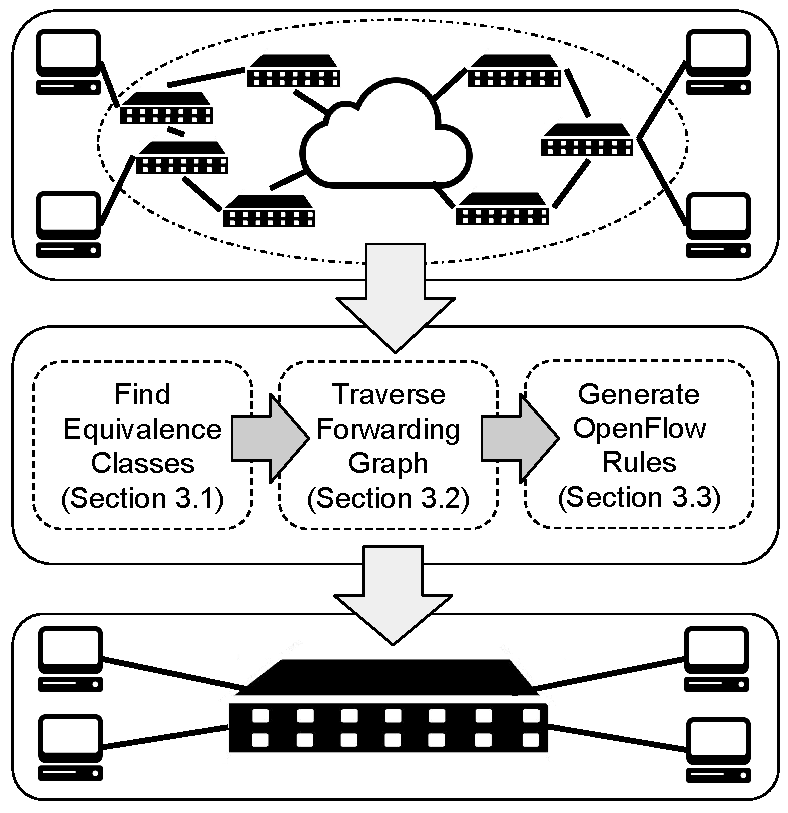
\includegraphics[scale=.6]{figures/BigSimOverview.pdf}
\caption{BigSim transforms a SDN network (controller is not shown for simplicity) to a
virtual OpenFlow switch without the loss of forwarding logic.}
\label{Fig:BigSimOverview}
\end{figure}

